\documentclass[11pt]{article}

\usepackage{amsmath, amsthm, amssymb, amsfonts}
\usepackage{thmtools}
\usepackage{graphicx}
\usepackage{setspace}
\usepackage{geometry}
\usepackage{float}
\usepackage{hyperref}
\usepackage[utf8]{inputenc}
\usepackage[english]{babel}
\usepackage{framed}
\usepackage[dvipsnames]{xcolor}
\usepackage[most]{tcolorbox}
\usepackage{minted}
\usepackage{enumitem}
\usepackage{subcaption}
\usepackage{csquotes}
\usepackage{indentfirst}
\usepackage[export]{adjustbox}
\usepackage{booktabs}
\usepackage{microtype}
\usepackage{fancyhdr}
\usepackage{cleveref}

\definecolor{LightGray}{RGB}{230, 230, 242}
\definecolor{LightOrange}{RGB}{255, 239, 213}
\definecolor{LightGreen}{RGB}{240, 255, 240}
\definecolor{MainBlue}{RGB}{0, 60, 113}

\newcommand{\HRule}[1]{\rule{\linewidth}{#1}}
\newcommand{\code}[1]{\texttt{#1}}

\newtcbtheorem[auto counter,number within=section]{algorithm}{Algorithm}{
  colback=LightOrange!20,
  colframe=LightOrange,
  colbacktitle=LightOrange,
  fonttitle=\bfseries\color{black},
  boxed title style={size=small,colframe=LightOrange},
}{alg}

\geometry{
  textheight=24.5cm,
  textwidth=15.75cm,
  top=2cm,
  headheight=12pt,
  headsep=20pt,
  footskip=20pt,
  marginparwidth=1.5cm
}

\setstretch{1.15}

\pagestyle{fancy}
\fancyhf{}
\fancyfoot[C]{\thepage}

\begin{document}

\begin{titlepage}
\begin{center}
  \vspace*{1cm}
  
\includegraphics[scale = 0.3]{img/IST_A.eps}
  
  \vspace{1.5cm}
  {\LARGE\textsc{Aprendizagem}}
  
  \vspace{0.7cm}
  {\LARGE\textsc{LEIC IST-UL}}
  
  \vspace{0.7cm}
  \HRule{1.5pt}
  \vspace{0.3cm}
  {\LARGE\textbf{\uppercase{Relatório - Merit Prize Challenge}}}
  \HRule{1.5pt}
  
  \vspace{2cm}
  
  \begin{minipage}{0.7\textwidth}
    \begin{flushleft}
      \large\textbf{Group 10:}\\[0.3cm]
      \large Gabriel Ferreira\\
      \large Irell Zane
    \end{flushleft}
  \end{minipage}%
  \begin{minipage}{0.3\textwidth}
    \begin{flushright}
      \large 107030\\
      \large 107161
    \end{flushright}
  \end{minipage}
  
  \vfill
  
  {\large\textbf{2024/2025 -- 1st Semester, P1}}
\end{center}
\end{titlepage}

\section{Logistic Regression Analysis}

We conducted a comprehensive analysis of logistic regression performance using both raw and standardized data to evaluate the impact of preprocessing on model effectiveness. The standardization process involved scaling the features to have zero mean and unit variance, which helps prevent features with larger scales from dominating the model's learning process.

\begin{table}[H]
\centering
\caption{Logistic Regression Performance Comparison}
\label{tab:log-accuracy}
\begin{tabular}{@{}lcc@{}}
\toprule
Preprocessing Method & Testing Accuracy & Training Accuracy \\ \midrule
Without Scaling & 97.66\% & 95.98\% \\
Standardized Data & 98.25\% & 98.74\% \\
\bottomrule
\end{tabular}
\end{table}

The results demonstrate that standardization led to improved performance across both training and testing datasets. The standardized model achieved a testing accuracy of 98.25\%, representing a significant improvement over the non-standardized version. This improvement suggests that feature scaling is crucial for this dataset, likely due to the varying scales of the original features.

\section{EM Clustering Analysis}

Our implementation of Expectation-Maximization (EM) clustering utilized \code{scikit-learn}'s \code{GaussianMixture} model. We evaluated clustering quality using silhouette scores across different numbers of clusters ($k \in [2,10]$) to determine the optimal cluster count for our dataset.

\begin{figure}[H]
  \centering
  \begin{minipage}{0.48\textwidth}
    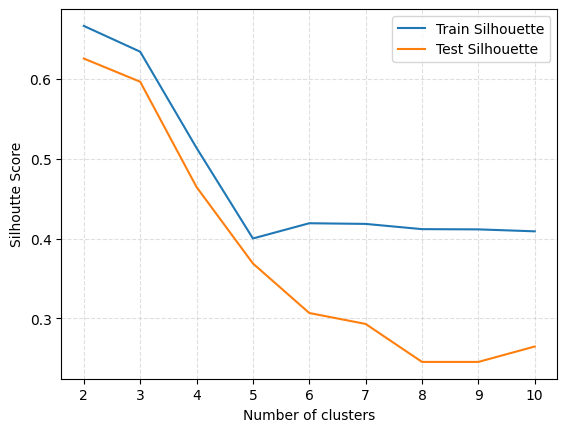
\includegraphics[width=\linewidth]{img/Silhouettes.png}
    \caption{Silhouette scores vs. cluster count}
    \label{fig:silhouette-score}
  \end{minipage}
  \hfill
  \begin{minipage}{0.48\textwidth}
    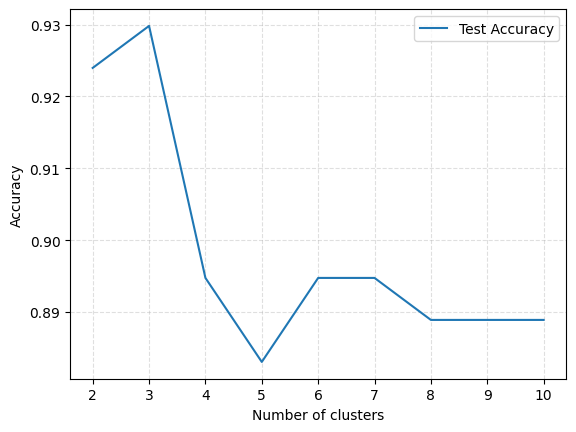
\includegraphics[width=\linewidth]{img/EMProbMapAccuracy.png}
    \caption{Logistic Reggression on the EM Probability Map}
    \label{fig:em-accuracy}
  \end{minipage}
\end{figure}

The silhouette analysis revealed several important trends:
\begin{itemize}
    \item A clear declining trend in clustering quality as the number of clusters increases
    \item Growing disparity between training and testing silhouette scores with higher cluster counts
    \item Optimal clustering achieved with k=2, yielding silhouette scores of 0.626 (testing) and 0.667 (training)
\end{itemize}

Upon analyzing the relationship between the number of clusters 
($k$) and both performance metrics - the Silhouette scores and
Logistic Regression accuracy on the mapped dataset - we can see
that there is a notable relation: For low numbers of clusters,
such as 2 and 3, both metrics show high values, and as the $k$
increases, there is a sharp decline in both the silhouette score
and the classification accuracy of the logistic model, which
seem to follow the same trajectory, suggesting that a higher
quality of clustering, as measured by the Silhouette score, is
conducive to a better logistic regression model.

Using $k=2$ or $k=3$ the EM algorithm effectively serves as a
dimensionality reduction technique, transforming the original
high-dimensional feature space (30 features) into a lower
dimensional feature space, while maintaining a high accuracy
on the logistic regression model.

\section{RBF Network Implementation}

Our Radial Basis Function (RBF) Network implementation consisted of three key layers:
\begin{enumerate}
    \item Input layer matching the dimension of observations
    \item Hidden layer corresponding to the number of clusters
    \item Output layer with a single neuron for binary classification
\end{enumerate}

The Gaussian Radial Basis Function employed in our network is defined as:
\begin{equation}
  \phi_k(x)=exp(-\gamma \cdot (x-\mu)^T\Sigma_k^{-1}(x-\mu))
\end{equation}

Initial implementation with $\gamma=\frac{1}{2}$ yielded low accuracies:
\begin{itemize}
    \item Train Accuracy: 0.6256281407035176
    \item Test Accuracy: 0.631578947368421
\end{itemize}
This was due to several challenges with the activation distributions:

\begin{figure}[H]
    \centering
    \begin{minipage}{0.48\textwidth}
        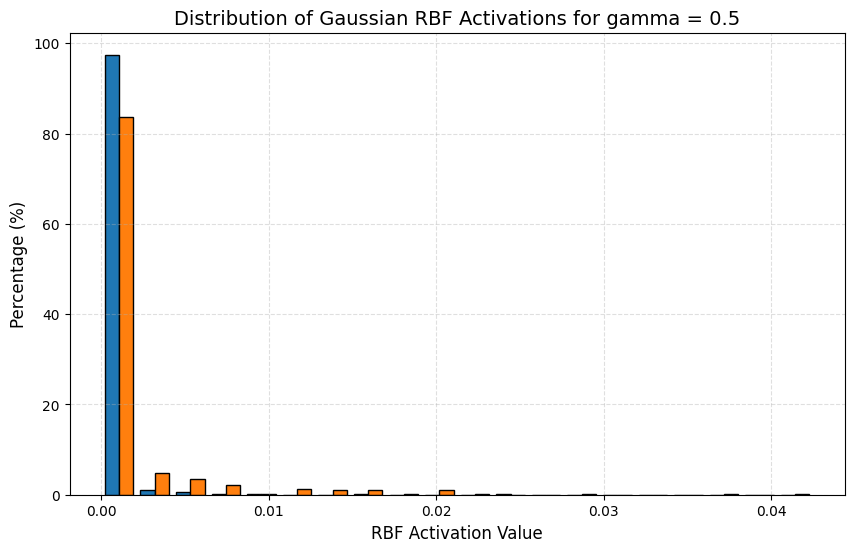
\includegraphics[width=\linewidth]{img/RBF_Activation_500.png}
        \caption{Hidden layer activation distribution ($\gamma=0.5$)}
    \end{minipage}
    \hfill
    \begin{minipage}{0.48\textwidth}
        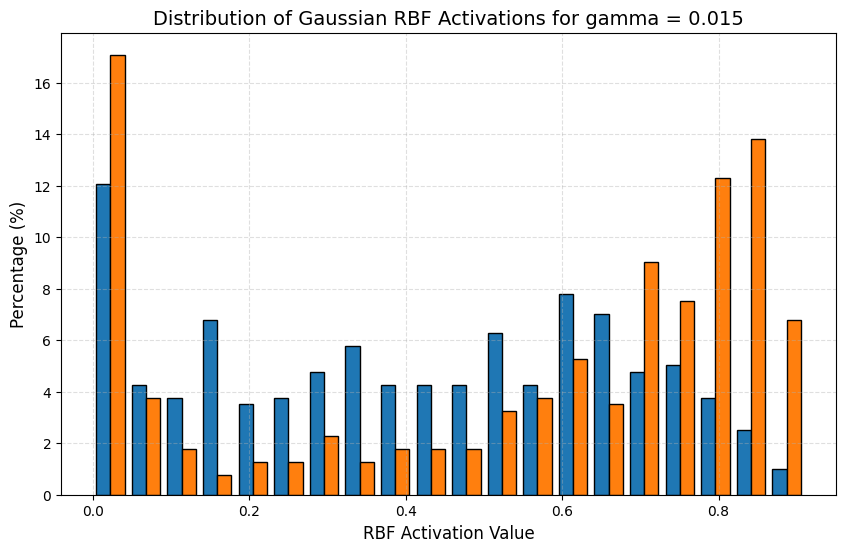
\includegraphics[width=\linewidth]{img/RBF_Activation_15.png}
        \caption{Hidden layer activation distribution ($\gamma=0.015$)}
    \end{minipage}
\end{figure}

The low accuracy was due to distances being too large, gamma being too low, and floating point precision issues. We experimented with different gamma values:
To address these challenges, we conducted extensive experimentation with different gamma values and implemented Normalized RBF:

\begin{figure}[H]
  \centering
  \begin{minipage}{0.48\textwidth}
    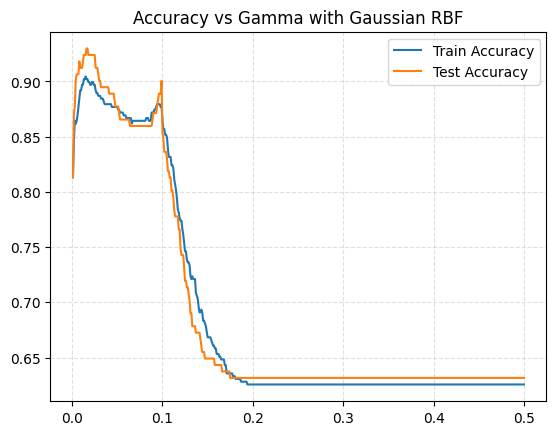
\includegraphics[width=\linewidth]{img/GammaHyperparameterTuning.png}
    \caption{RBF Network gamma parameter tuning results}
  \end{minipage}
  \hfill
  \begin{minipage}{0.48\textwidth}
    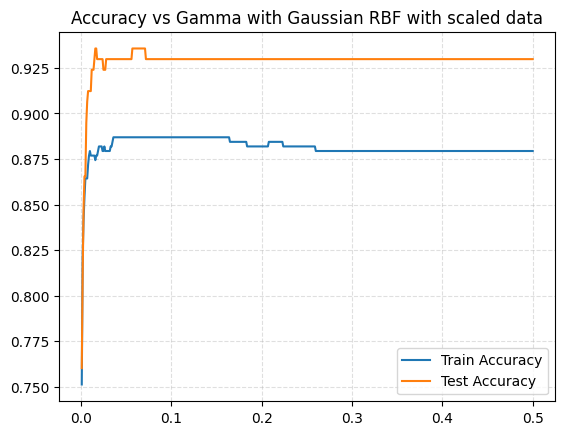
\includegraphics[width=\linewidth]{img/NormGammaHyperparameterTuning.png}
    \caption{Normalized RBF Network gamma tuning results}
  \end{minipage}
\end{figure}

The Normalized RBF (NRBF) implementation achieved several improvements:
\begin{itemize}
    \item Increased testing accuracy to 92.96\% with $\gamma=0.5$
    \item Reduced sensitivity to gamma parameter selection
    \item More stable and consistent performance across different configurations
    \item Better distribution of activation values, leading to improved learning
\end{itemize}

The NRBF distributions are discriminative in that there is as much small activations as there are large, (Suggesting points that are part of a cluster and points that are not):

\begin{figure}[H]
  \centering
  \begin{subfigure}{0.45\linewidth}
      \centering
      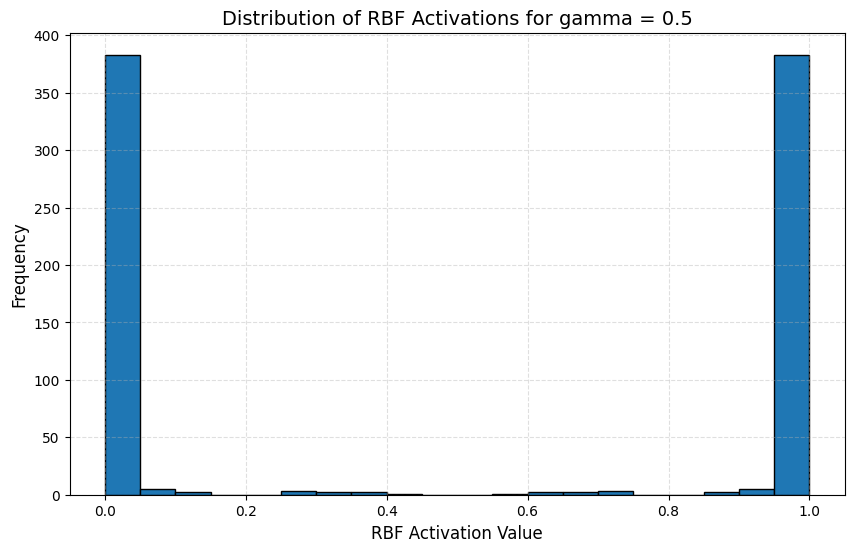
\includegraphics[width=\linewidth]{img/NRBF_Activation_500.png}
      \caption{$\gamma=0.5$}
  \end{subfigure}
  \hfill
  \begin{subfigure}{0.45\linewidth}
      \centering
      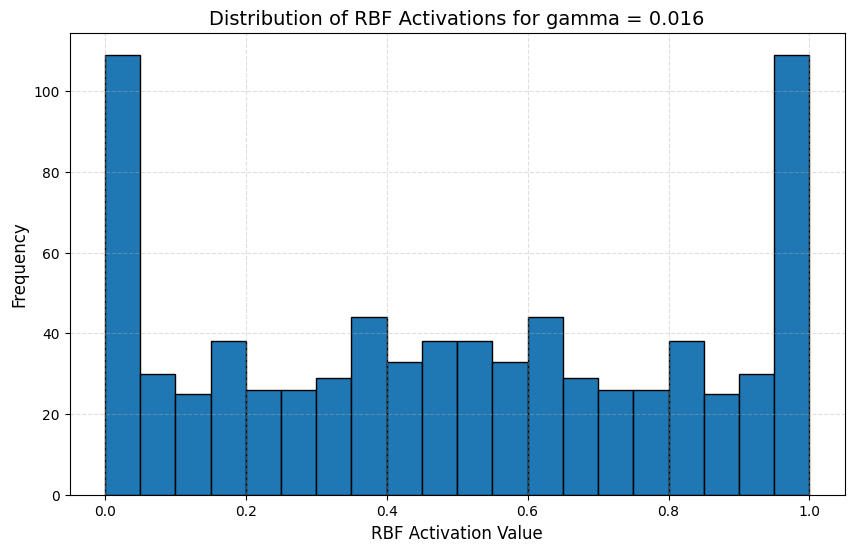
\includegraphics[width=\linewidth]{img/NRBF_Activation_16.png}
      \caption{$\gamma=0.036$}
      \label{fig:nrbf-dist-16}
  \end{subfigure}
  \caption{Hidden layer activation value distribution}
  \label{fig:nrbf-dist}
\end{figure}

We also explored alternative basis functions. Here is the Linear RBF approach:

\begin{figure}[H]
  \centering
  \begin{minipage}{0.48\textwidth}
    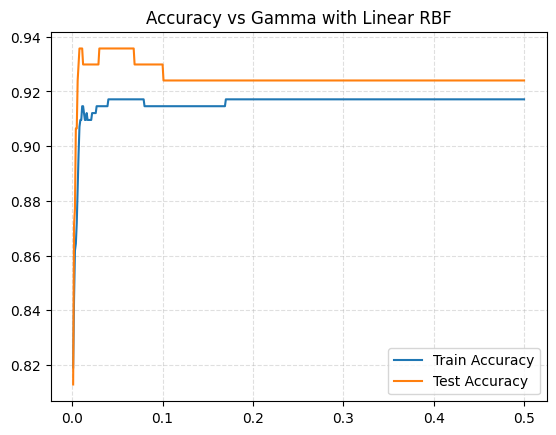
\includegraphics[width=\linewidth]{img/LinearRBF.png}
    \caption{Linear RBF performance analysis}
  \end{minipage}
  \hfill
  \begin{minipage}{0.48\textwidth}
    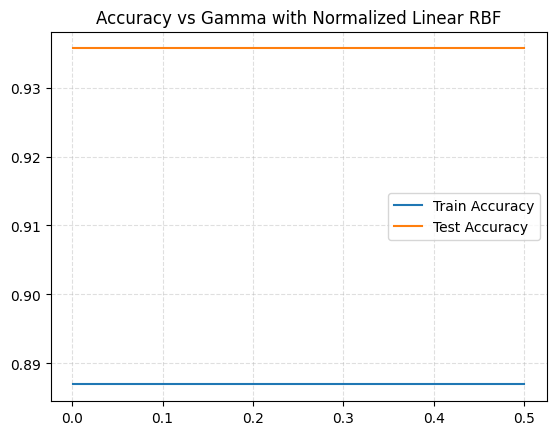
\includegraphics[width=\linewidth]{img/LinearNRBF.png}
    \caption{Normalized Linear RBF performance}
  \end{minipage}
\end{figure}

The Linear RBF implementation showed promising results, often outperforming the Gaussian RBF in terms of both accuracy and stability.

\section{Comparative Analysis and Conclusions}

Our comprehensive evaluation of different approaches revealed several key insights about both the models and the underlying data structure:

\begin{table}[H]
\centering
\caption{Model Performance Summary}
\begin{tabular}{@{}lc@{}}
\toprule
Model                              & Testing Accuracy \\ \midrule
Logistic Regression (Standardized) & 98.25\%          \\
EM Probability Mapping ($k=2$)     & 92.40\%          \\
Gaussian RBF Network               & 92.40\%          \\
Normalized Gaussian RBF Network    & 92.96\%          \\
Linear RBF Network                 & 93.57\%          \\
Normalized Linear RBF Network      & 93.57\%          \\ \bottomrule
\end{tabular}
\end{table}

Key findings from our analysis:
\begin{itemize}
    \item Logistic regression's high accuracy (98.25\%) suggests predominantly linear decision boundaries in the feature space
    \item EM clustering successfully reduced dimensionality while preserving most of the discriminative information
    \item The normalized RBF approach demonstrated robust performance across various parameter settings
    \item Preprocessing and normalization proved essential for optimal performance across all methods
    \item The dataset exhibits natural binary structure, aligning well with the classification objective
\end{itemize}

The practical implications of our findings include:
\begin{enumerate}
    \item EM clustering with k=2 provides an effective approach for dimensionality reduction while maintaining good classification performance
    \item Normalized RBF networks offer stable performance without requiring extensive parameter tuning
    \item Feature standardization consistently improves model performance across different approaches
    \item The choice between methods involves a trade-off between accuracy and computational complexity
\end{enumerate}

\bibliography{references}
Luis Sa-Couto and Andreas Miroslaus Wichert, 
\textit{Machine Learning - A Journey To Deep Learning: With Exercises And Answers}, 
International series of monographs on physics, 
World Scientific Pub Co Inc, 2021, ISBN: 9789811234057.
\bibliographystyle{plain}

\end{document}